%=========================================
% 	   Architektur						 =
%=========================================
\section{Architektur}

\textit{Open for extension, closed for modification} \footnote{Robert C.Martin, \textit{The Open/
Closed Principle}} - Um einen hohen Grad an Flexibilität und Wartbarkeit zu erzielen, sowie eine 
Abhängigkeit von konkreten Klassen zu vermeiden, ist die Wahl eines geeigneten Architekturmusters 
essentiell. Besonders für Webanwendungen bietet sich eine \ac{MVC} Architektur an, um die 
Interaktion zwischen Client und Server zu abstrahieren und die Kommunikation transparent zu gestalten.
\\\\
Bei dem klassischen \acs{MVC} unterscheidet man zwischen den Komponenten:
\begin{itemize}
  \item Das \textbf{Model} dient als Verarbeitungskomponente und enthält Daten sowie Kernfunktionalität.
  \item Die \textbf{View} stellt die Ausgabekomponente dar. Sie zeigt dem Anwender Informationen, welche vom Model bezogen werden.
  \item Der \textbf{Controller} steuert als Kontrollkomponente alle Eingaben und vermittelt diese zwischen Model und View.
\end{itemize}
Im folgenden Abschnitt wird die Umsetzung des \acs{MVC}-Musters in Spring betrachtet. Insbesondere wird 
dabei klar, wie das Muster im Kontext \textit{Web} funktioniert und wie dies die Anwendung hinsichtlich 
ihrer Erweiterbarkeit und Wartbarkeit verbessert.
\subsection{Das Spring Web MVC Framework}
Spring unterstützt die \acs{MVC} Architektur als integralen Bestandteil des Frameworks. Basierend auf einigen Java-Konzepten wie beispielsweise \textit{Annotations} oder \textit{Dependency Injection} können somit komplexe Webanwendungen realisiert werden. Die Implementierung erfolgt dabei in leicht abgewandelter Struktur: \\
\begin{figure}[bth] 
  \centering
  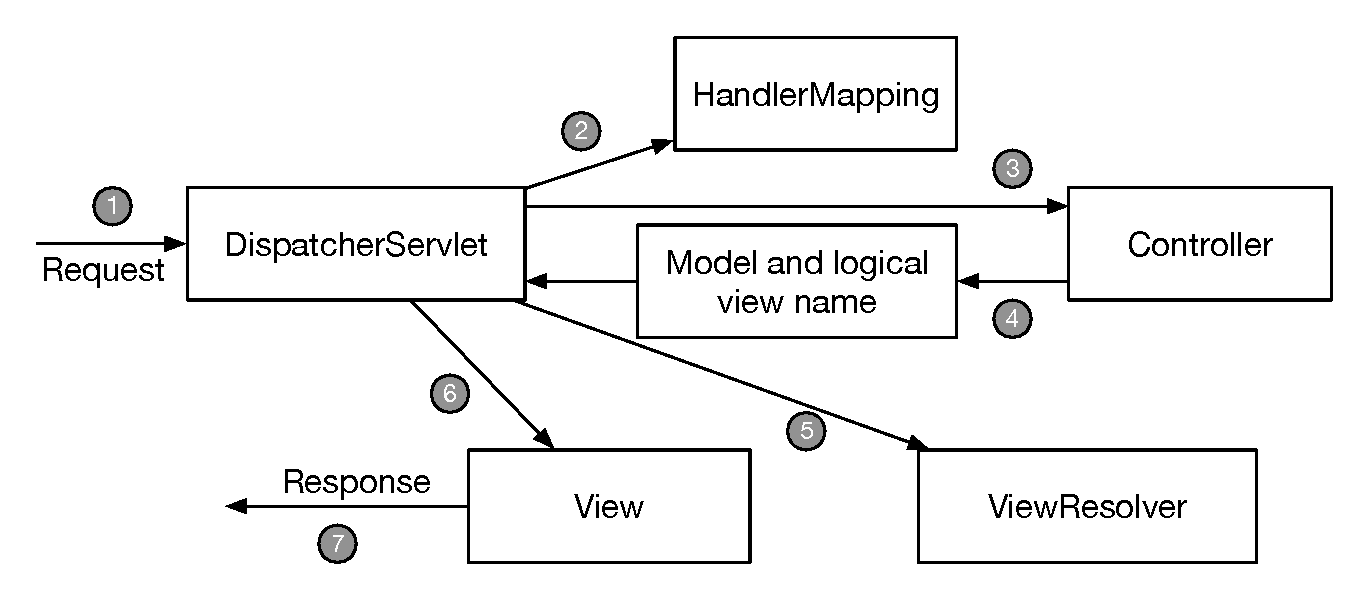
\includegraphics[width=0.8\textwidth]{Graphics/spring_mvc}
  \caption{Komponenten in Spring MVC}
\end{figure}
\newpage
Das \texttt{Dispatcher Servlet} stellt hierbei das zentrale Element der Architektur dar. Dieses fungiert als Fassade, nimmt Anfragen vom Client entgegen und verteilt diese auf die jeweils zuständigen Controller. Die dabei notwendige Zuordnung zwischen Eingabe und Kontrollkomponente wird von einem \texttt{HandlerMapper} übernommen. Der \texttt{Controller} nimmt nun die Eingabe entgegen und verarbeitet die Daten. Meist werden dabei sogenannte \texttt{Service}-Klassen referenziert, welche die zur Berechnung notwendige Geschäftslogik enthalten. Werden bei der Datenverarbeitung Daten verändert oder erzeugt, so wird das zugehörige \texttt{Model} angepasst. Der \texttt{Controller} leitet dann dessen Referenz zusammen mit einem \texttt{View Name} an das \texttt{Dispatcher Servlet}. Der \texttt{View Name} kann nun von einem \texttt{View Resolver} mit einer konkrete Implementierung identifiziert werden. Dies kann beispielsweise in Form einer \acs{JSP} geschehen. Der \texttt{View} rendert schließlich die Daten und liefert ein \texttt{Response Object} zurück.